\chapter{Evaluation}

This section is focused on the empirical evaluation of Spazio as a QoS
scheduler. I aim to evaluate Spazio's:
\begin{itemize}
    \item Overhead - the computational overhead introduced by the Spazio Pods on
        the Nodes
    \item Resource Utilisation - measured resource utilisation during various
        workloads
    \item Throughput - the time it takes for Jobs of various sizes and workloads
        to complete
    \item Workload Isolation - the impact of scheduling decisions on long
        running Pods within the cluster
\end{itemize}
Throughout this evaluation, I will compare Spazio against
\texttt{kube-scheduler}, an industry-standard scheduler that was built upon the
lessons learnt from Borg \cite{}. \texttt{kube-scheduler} is the default
scheduler in Kubernetes, and thus, has been thoroughly designed to be as optimal
as possible. As \texttt{kube-scheduler} is a Pod description-based scheduler, I
test with mutliple different resource requests to highlight how the performance
achieved can vary depending on description.

\section{Evaluation Setup}
These experiments ran on a Kubernetes cluster containing 20 virtual machines
(VMs) running on the Xen hypervisor. One of the machines is used as the master
Node, and the rest are worker Nodes. The master Node contains all the Pods in
the control plane, and during the evaluation of Spazio, it contains the Spazio
Scheduler and Aggregation Server. Each VM features four Intel Xeon Gold 6142
CPUs \@ 2.60Ghz with 8 GB of RAM running Ubuntu 24.04.2 LTS. Each CPU has a
single core with hyperthreading disabled. When running \texttt{kubectl describe
nodes}, each Node advertises $4000$ milli-CPU seconds and 8GB of RAM.

During the evaluation, I use a Prometheus deployment \cite{} to collect various
statistics, such as running Pod count, resource utilisation and Kubernetes
object completions.

\section{Spazio Overhead}
To measure the overhead incurred from running the Spazio pods on the Nodes, I
compared the completion time of Jobs when running on Nodes with and without the
Spazio deployment. I considered easuring resource utilisation on a Node with
just the Spazio Pod running, but much of the behaviour of the
Spazio Pod occurs during container events. As a result, the measured overhead
would not represent the entire impact of the Spazio Pod. Instead, by measuring
the overhead over Jobs, we aggregate the impact of Spazio across multiple
container events, providing a more holistic view of its impact.

\begin{table}[H]
\centering
    \begin{tabular}{|c|c|}
    \hline
    \textbf{Number of Pods} & \textbf{\% Overhead with Spazio} \\
    \hline
        100 & -2.33 $\pm$ 3.29 \\
        250 & -1.19 $\pm$ 2.44 \\
        500 & 4.84  $\pm$ 1.25 \\
        750 & 1.69  $\pm$ 0.42 \\
        1000 & 2.27  $\pm$ 0.66 \\
    \hline
    \end{tabular}
    \label{tab:overhead}
    \caption{The overhead incurred when running Spazio Pods on Nodes during the
    executing of Jobs with varying Pod counts. Each Pod executed
    \texttt{bpi(2000)} and requested 200 milliseconds of CPU time.}
\end{table}

To measure Spazio's overhead, I compared the Completion time of varying
sized Jobs, each Pod executing \texttt{bpi(2000)}, with and without Spazio Pods
running on all the Nodes. Table \ref{tab:overhead} presents the relative change
in Job Completion time with Spazio Pods running on the Nodes. We can see that
the Job Completion time of smaller Jobs are more noisy, therefore, resulting in
an observed decrease in Job Completion times. However, with larger and more
stable Jobs, the overhead from Spazio is more visible. From these observations
we can conclude that Spazio has $\approx$ 2\% overhead.
%
% For any practical projects, you should almost certainly have some kind
% of evaluation, and it's often useful to separate this out into its own
% chapter.
\section{Resource Utilisation}
This section investigates the resource utilisation when scheduling with Spazio.
For this experiment, I measured CPU and memory utilisation, as these are common
metrics used to evaluate schedulers.


\begin{figure}[H]
    \centering
    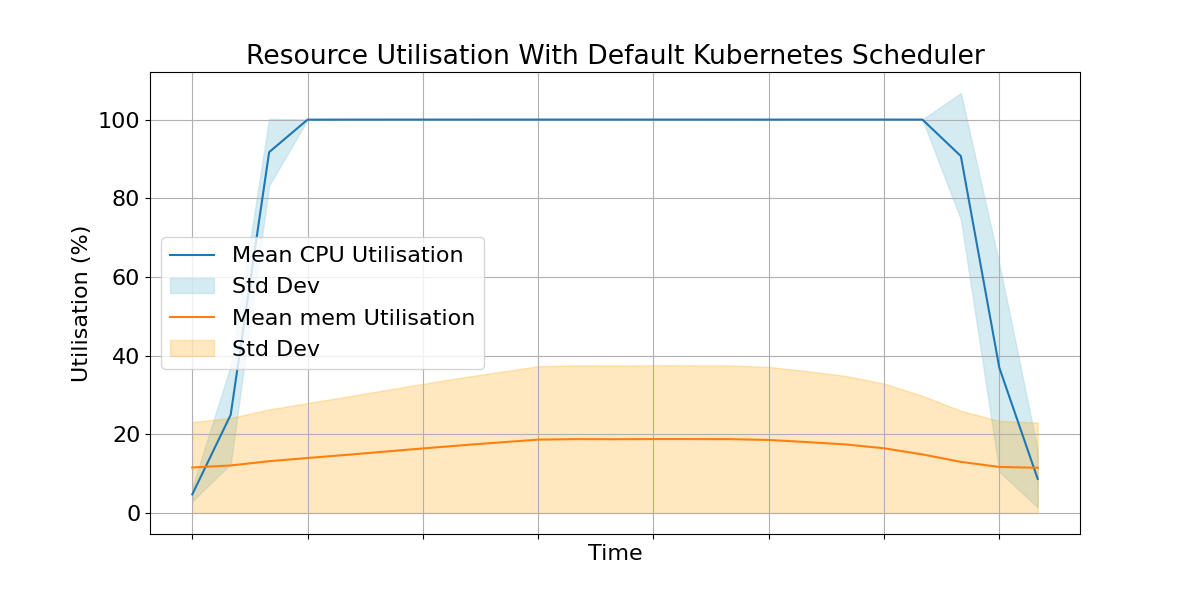
\includegraphics[width=\textwidth]{images/pi-2000-1000x-pod-kube-util.png}\\
    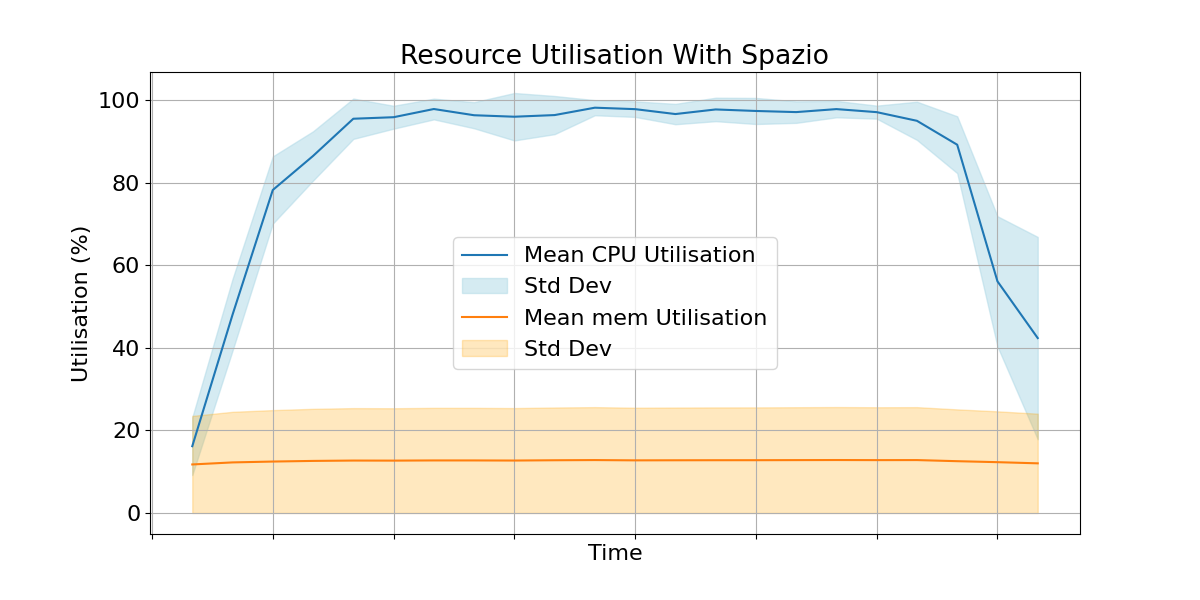
\includegraphics[width=\textwidth]{images/pi-2000-1000x-pod-spazio-util.png}
    \caption{The resource utilisation when scheduling a Job with 1000 Pods
    executing \texttt{bpi(2000)}. The top figure gives the resource utilisation
    when scheduling with the default Kubernetes scheduler. The bottom figure
    gives the resource utilisation when scheduling with SPAZIO.}
    \label{fig:pi-2000-1000x-pod-util}
\end{figure}

Figure \ref{fig:pi-2000-1000x-pod-util} shows the resource utilisation running
only running a CPU-focused Job. The default Kubernetes scheduler achieves 100\%
CPU utilisation. This is because each Pod requests 100 milliseconds of CPU time
and therefore, the default scheduler allocates them all at once evenly across
the Nodes ($\approx$ 50 Pods per Node). This allocation results in very high CPU
contention, and we can even observe an increase in memory usage. This contrasts
SPAZIO, which still achieves a $> 95\%$ utilisation but a constant memory
utilisation.

\section{Throughput}
Job Completion is the time it takes for all of the Pods in a Job deployment to
complete. The more optimal the allocation of Pods, the faster it takes for all
the Pods to complete, reducing the Job Completion. This property makes it a
useful indicator of throughput. To evaluate thoroughly evaluate SPAZIO, I
measure the Job Completion of various workloads.

\subsection{CPU-Focused Workloads}
In this experiment, I use a Job that specifies Pods that execute
\texttt{bpi(2000)}. This simple workload allows us to observe how each scheduler
handles CPU-focused workloads. To ensure fairness when evaluating against the
default Kubernetes scheduler, I used different CPU requests to show how
different Pod-descriptions could impact the performance of the default
scheduler. The results are given in Table \ref{tab:pi-2000-throughput}

\begin{table}[H]
\centering
    \begin{tabular}{|l|r|c|c|c|c|c|}
    \hline
    \textbf{Scheduler} & \textbf{Requested} & \multicolumn{5}{c|}{\textbf{Job Completion (s)}} \\
    \cline{2-7}
    &  \textbf{CPU} & \textbf{100 Pods} & \textbf{250 Pods} & \textbf{500 Pods} & \textbf{750 Pods} & \textbf{1000 Pods} \\
    \hline
    Default & 100m & 15.7 $\pm$ 0.6 & 31.7 $\pm$ 2.1 & 56 $\pm$ 1.7 & 84.7 $\pm$
        0.6 & 112 $\pm$ 0.0 \\
    Default & 200m & 15.7 $\pm$ 0.7 & 30.7 $\pm$ 0.6 & 55 $\pm$ 1 & 79 $\pm$ 0.0
        & 103 $\pm$ 1 \\
    Default & 500m & 15.7 $\pm$ 1.2 & 32 $\pm$ 2.6 & 57.7 $\pm$ 0.6 & 81 $\pm$ 2
        & 104 $\pm$ 2.1 \\
    Default & 1000m & 21 $\pm$ 2.0 & 54.7 $\pm$ 0.6 & 96 $\pm$ 2.6 & 133 $\pm$
        0.6 & 175 $\pm$ 1 \\
    Spazio &  & 20.3 $\pm$ 0.6 & 35.3 $\pm$ 0.6 & 60.3 $\pm$ 2.5 & 89 $\pm$ 2 &
        109$\pm$ 1 \\
    \hline
    \end{tabular}
    \caption{Job Completion of Job deployments with different Pod counts. Each
    Pod executed \texttt{bpi(2000)}. For the default scheduler, the requested
    resources are also given}
    \label{tab:pi-2000-throughput}
\end{table}

From Table \ref{tab:pi-2000-throughput}, we can see how much the performance of
the default scheduler varies depending on the amount of CPU time requested.
Over-estimating requests can result in the CPU being underutilised, while
under-estimating can result in too many Pods running on a Node at once. With
SPAZIO, we observed only observed a 10\% reduction in Job Completion time. This
can be attributed to its use of telemetric data: CPU utilisation amd CPU
Pressure. In Section \ref{sec:issue-with-util}, I investigated these metrics and
showed how with \texttt{bpi(2000)} Pods, these metrics indicated full capacity
when running 4-8 Pods. As the capacity signal of a Node is tied to these
metrics, the Node's will never advertise more capacity than $\approx$ 8 Nodes.

\subsection{Memory-Focused Workloads}
In this experiment, I use a Job that specifies Pods that performed a small ML
workload. This workload uses a significant amount of memory, which unlike CPU,
must be carefully handled. If we increase the number of processes on a
fully-utilised CPU, it only results in each process having a smaller portion of
CPU time and degrading its performance. On the other hand, memory is less
forgiving as once memory runs out, the kernel begins OOM killing processes. This
be detrimental to Job Completion, as terminated Pods results in wasted
computations. The Job Completions from the experiment are given in Table
\ref{tab:ml-throughput}

\begin{table}[H]
\centering
    \begin{tabular}{|l|r|r|c|c|}
    \hline
    \textbf{Scheduler} & \multicolumn{2}{c|}{\textbf{Requested}} &
        \multicolumn{2}{c|}{\textbf{Job Completion (s)}} \\ \cline{2-5}
    &  \textbf{CPU} & \textbf{Memory} & \textbf{100 Pods} & \textbf{200 Pods} \\
    \hline
        Default & 200m & 750Mi & 153$\pm$ 12.5 & 362 $\pm$ 20.4\\
        SPAZIO &  &  & 142 $\pm$ 7.0 & 254 $\pm$ 5.03 \\
    \hline
    \end{tabular}
    \caption{Job Completion of Job deployments with different Pod counts. Each
    Pod executed a small ML workload. For the default scheduler, the requested
    resources are also given}
    \label{tab:ml-throughput}
\end{table}

\subsection{Mixed Workloads}
In this experiment, I deployed the two Jobs defined above: a short-lived
CPU-focused workload and a longer running ML workload. This experiment evaluates
how SPAZIO handles more than one type of workload. During the experiments, the
\texttt{bpi(2000)} Pods requested 100 milliseconds of CPU time and the ML
workload requested 200 milliseconds of CPU time and 750Mi of memory. To
thoroughly evaluate SPAZIO in this scenario, I varied the distribution of Pods
from each Job. The observed Job Completions are given in Table
\ref{tab:mixed-throughput}.

\begin{table}[H]
\centering
    \begin{tabular}{|l|c|c|c|}
    \hline
    \textbf{Scheduler} & \multicolumn{2}{c|}{\textbf{Job Size}} &
        \textbf{Job Completion (s)} \\ \cline{2-3}
        &  \texttt{bpi(2000)} & \texttt{ML} & \\
    \hline
        Default & 500 & 20 & 100.7 $\pm$ 9.01 \\
        SPAZIO & 500 & 20 & 88.7 $\pm$ 2.5 \\
        Default & 250 & 50 & 118 $\pm$ 4.58 \\
        SPAZIO & 250 & 50 & 115.7 $\pm$ 0.58 \\
        Default & 100 & 100 & 149 $\pm$ 0.0 \\
        SPAZIO & 100 & 100 & 192 $\pm$ 4.0 \\
    \hline
    \end{tabular}
    \caption{Job Completion of multi-resource Job deployments with different Pod
    counts. For the default scheduler, \texttt{bpi(2000)} Pods requested 100
    milliseconds of CPU and ML Pods requested 200 milliseconds CPU and 750Mi of
    memory}
    \label{tab:mixed-throughput}
\end{table}

\subsection{Pod Completions}
Due to Spazio's lackluster throughput, I decided to investigate distribution of
Pods across Nodes and how it impacted Pod Completion times.

\begin{figure}[H]
    \centering
    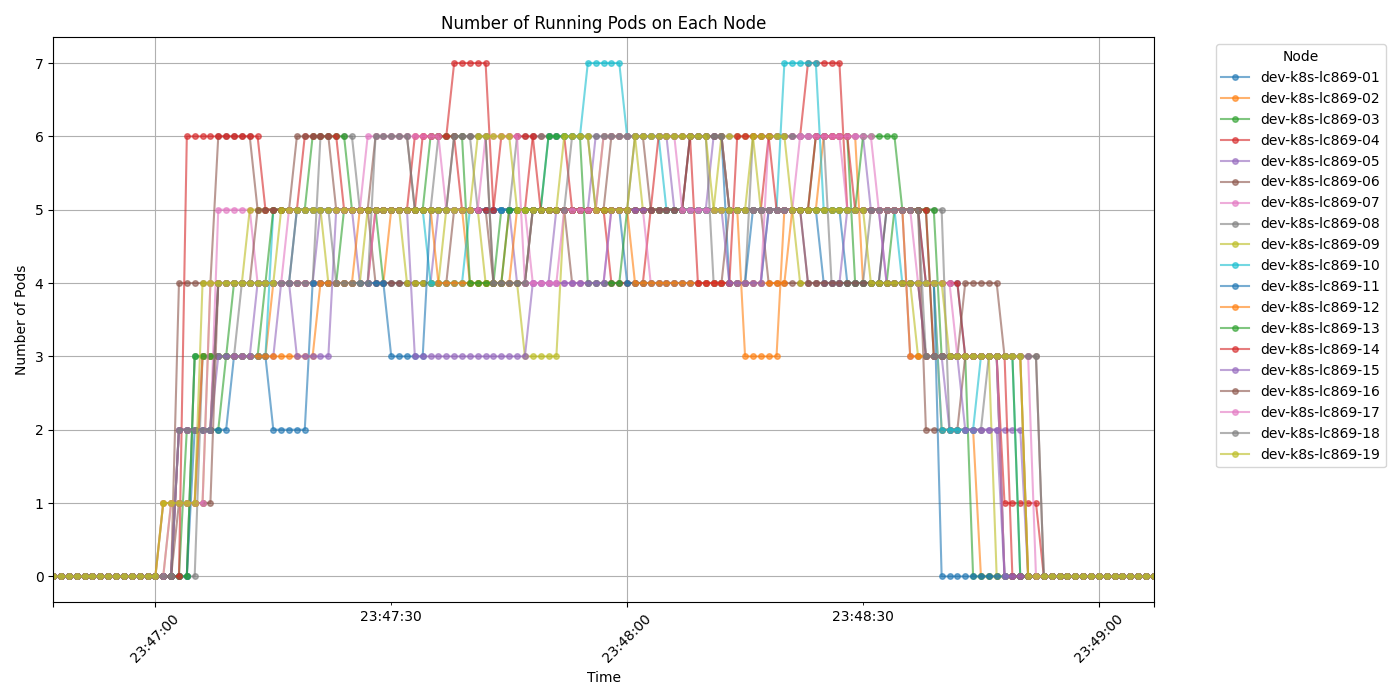
\includegraphics[width=\textwidth]{images/pi-2000-1000x-pod-running.png}
    \caption{The number of \texttt{bpi(2000)} Pods running on a Node during the
    execution of a Job with 1000 Pods.}
    \label{fig:pi-2000-1000x-pod-running}
\end{figure}

\begin{figure}[H]
    \centering
    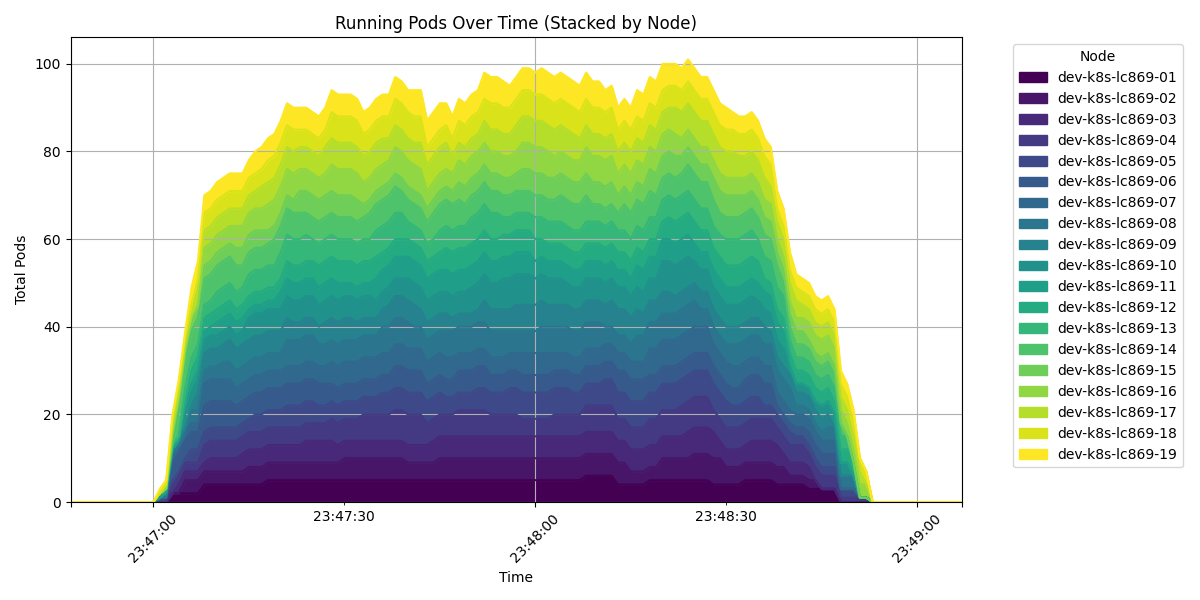
\includegraphics[width=\textwidth]{images/pi-2000-1000x-pod-running-stacked.png}
    \caption{The distribution of Pod Completion during the execution of a Job
    with 1000 \texttt{bpi(2000)} Pods.}
    \label{fig:pi-2000-1000x-pod-completion}
\end{figure}

TODO: WHICH SHOULD I USE THE LINE GRAPH OR THE STACKED GRAPH

\begin{figure}[H]
    \centering
    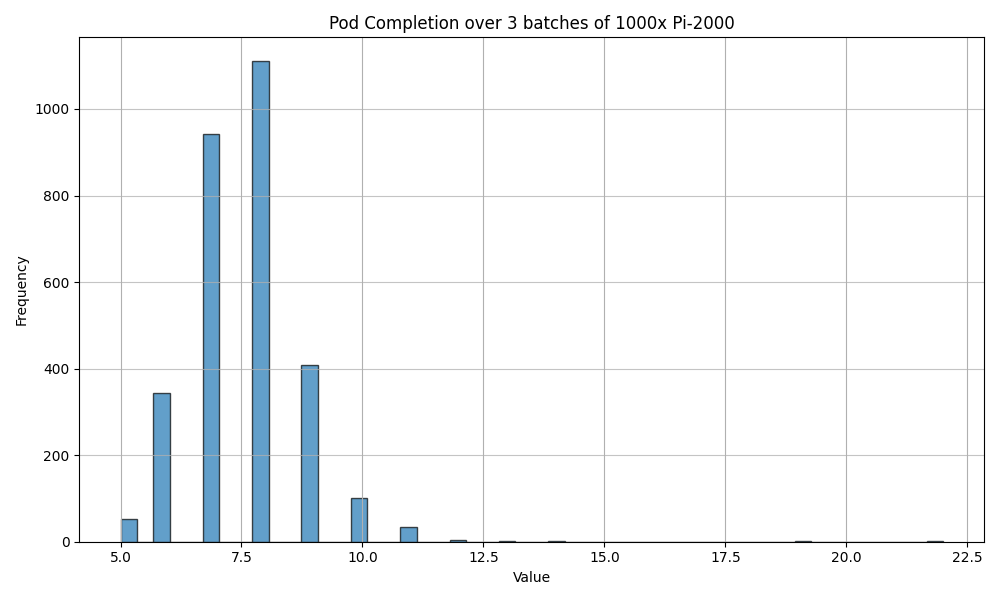
\includegraphics[width=\textwidth]{images/pi-2000-1000x-pod-completion.png}
    \caption{The distribution of Pod Completion during the execution of a Job
    with 1000 \texttt{bpi(2000)} Pods.}
    \label{fig:pi-2000-1000x-pod-completion}
\end{figure}

\section{Workload Isolation}
To evaluate Spazio's QoS, I investigated how its scheduling decisions impact the
performance of already running Pods. For this experiment, I had a Pod running on
a worker Node, while another Pod periodically sent HTTP GET requests. This
polling Pod would then measure latency of the response. I then scheduled a Job
of 1000 Pods executing \texttt{bpi(2000)} across the cluster and measured how
the response latency changed.

\begin{table}[h!]
\centering
    \begin{tabular}{|l|c|c|c|c|c|c|}
    \hline
    \textbf{Scenario} & \multicolumn{6}{c|}{\textbf{Response Latency (ms)}} \\
    \cline{2-7}
    & \textbf{Min} & \textbf{Med} & \textbf{P90} & \textbf{P95} & \textbf{P99} & \textbf{Max} \\
    \hline
    Baseline & 0.99 & 3.04 & 3.78 & 4.00 & 4.47 & 8.32 \\
    Default Scheduler & 1.07 & 10.06 & 18.61 & 22.28 & 28.82 & 54.49\\
    Spazio  & 1.00 & 2.48 & 6.09 & 7.82 & 10.53 & 17.39\\
    \hline
    \end{tabular}
    \caption{Job Completion of Job deployments with different Pod counts. This
    workload contained an event combination of Pods executing
    \texttt{bpi(2000)}, \texttt{bpi(4000)}, \texttt{bpi(6000)}. For the default
    scheduler, the requested resources are also given}
    \label{tab:pi-mixed-throughput}
\end{table}

\section{Limitation}
\begin{tcolorbox}[boxsep=0mm,left=2.5mm,right=2.5mm]
    \textbf{Limitations:} {\em In this section, I will go over the limitations
    of the system. I will highlight how certain metrics like CPU-Utilisations
    don't give any more information once saturated. I will also have to mention
    how due to the sub-linear pod completion time, the Kubernetes scheduler is
    able to achieve higher job throughput by packing more pods into nodes.
    }
\end{tcolorbox}

\section{Summary}
\begin{tcolorbox}[boxsep=0mm,left=2.5mm,right=2.5mm]
    \textbf{Summary:} {\em In this section, I will summarise the results of my
    evaluation section, highlighting key findings and reasoning.
    }
\end{tcolorbox}

